\documentclass{beamer}
\usetheme{metropolis}
\usepackage{ctex}
\usepackage{caption}
\usepackage{subfigure}

\title{Item-Based Collaborative Filtering}
\date{\today}
\author{Yang LI}
\institute{School of Software Engineering, Tongji University}

\begin{document}
  \maketitle
  \section{Visualization}
  \begin{frame}{Item-Count Chart}
    \begin{figure}
    \centering
    \subfigure{
      \begin{minipage}{0.45\linewidth}
        \centering
        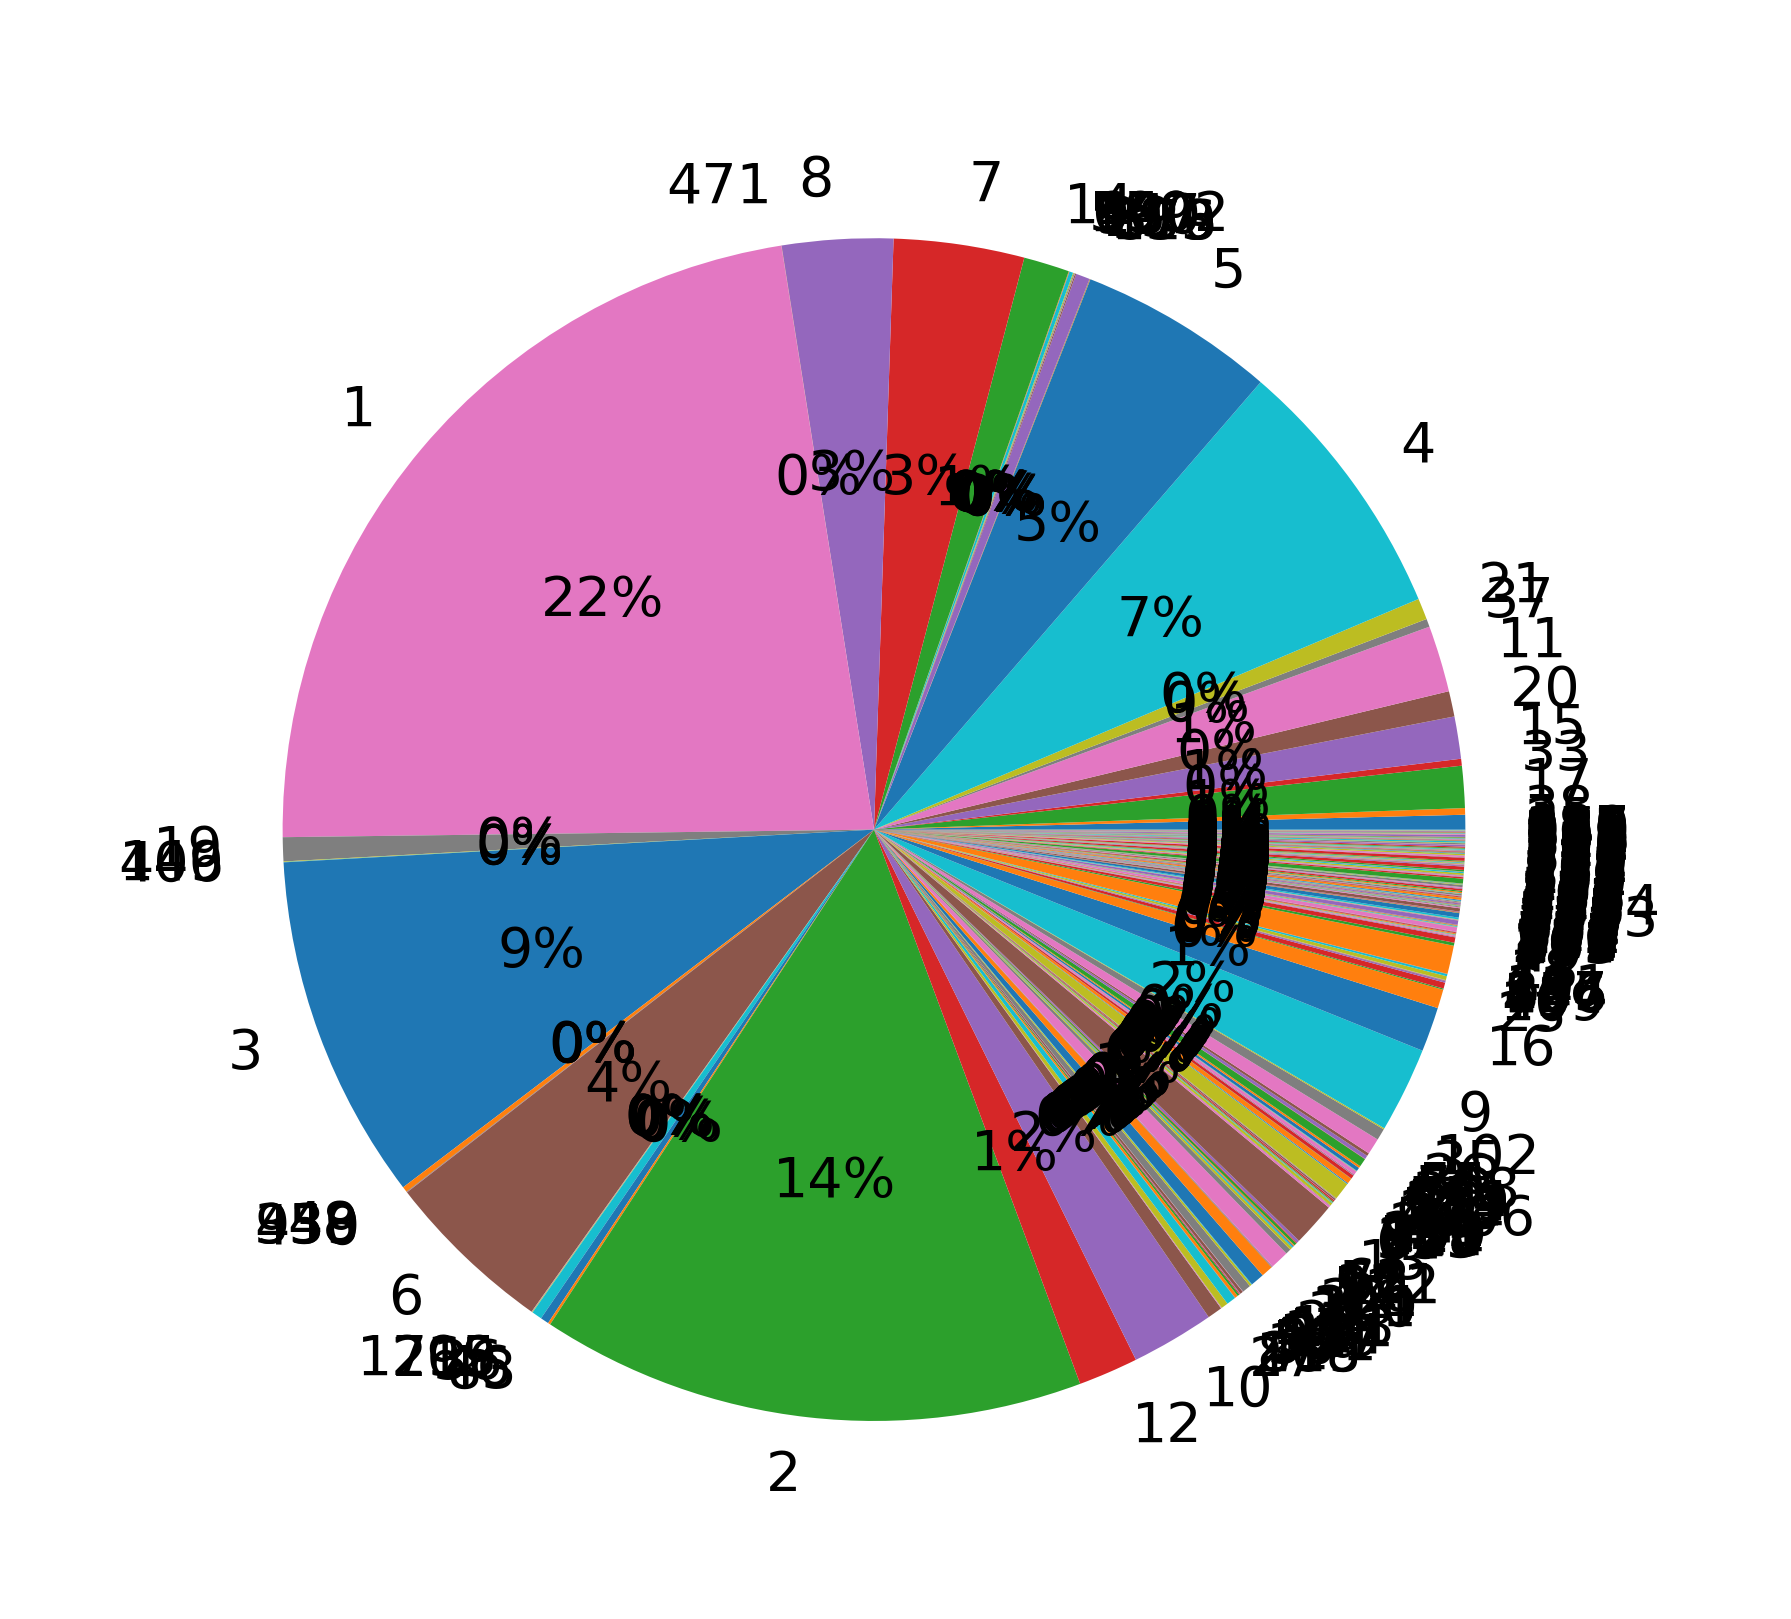
\includegraphics[width=2.3in]{../train_visualization_item}
        \caption{train\_item}
      \end{minipage}
    }
    \subfigure{
      \begin{minipage}{0.45\linewidth}
        \centering
        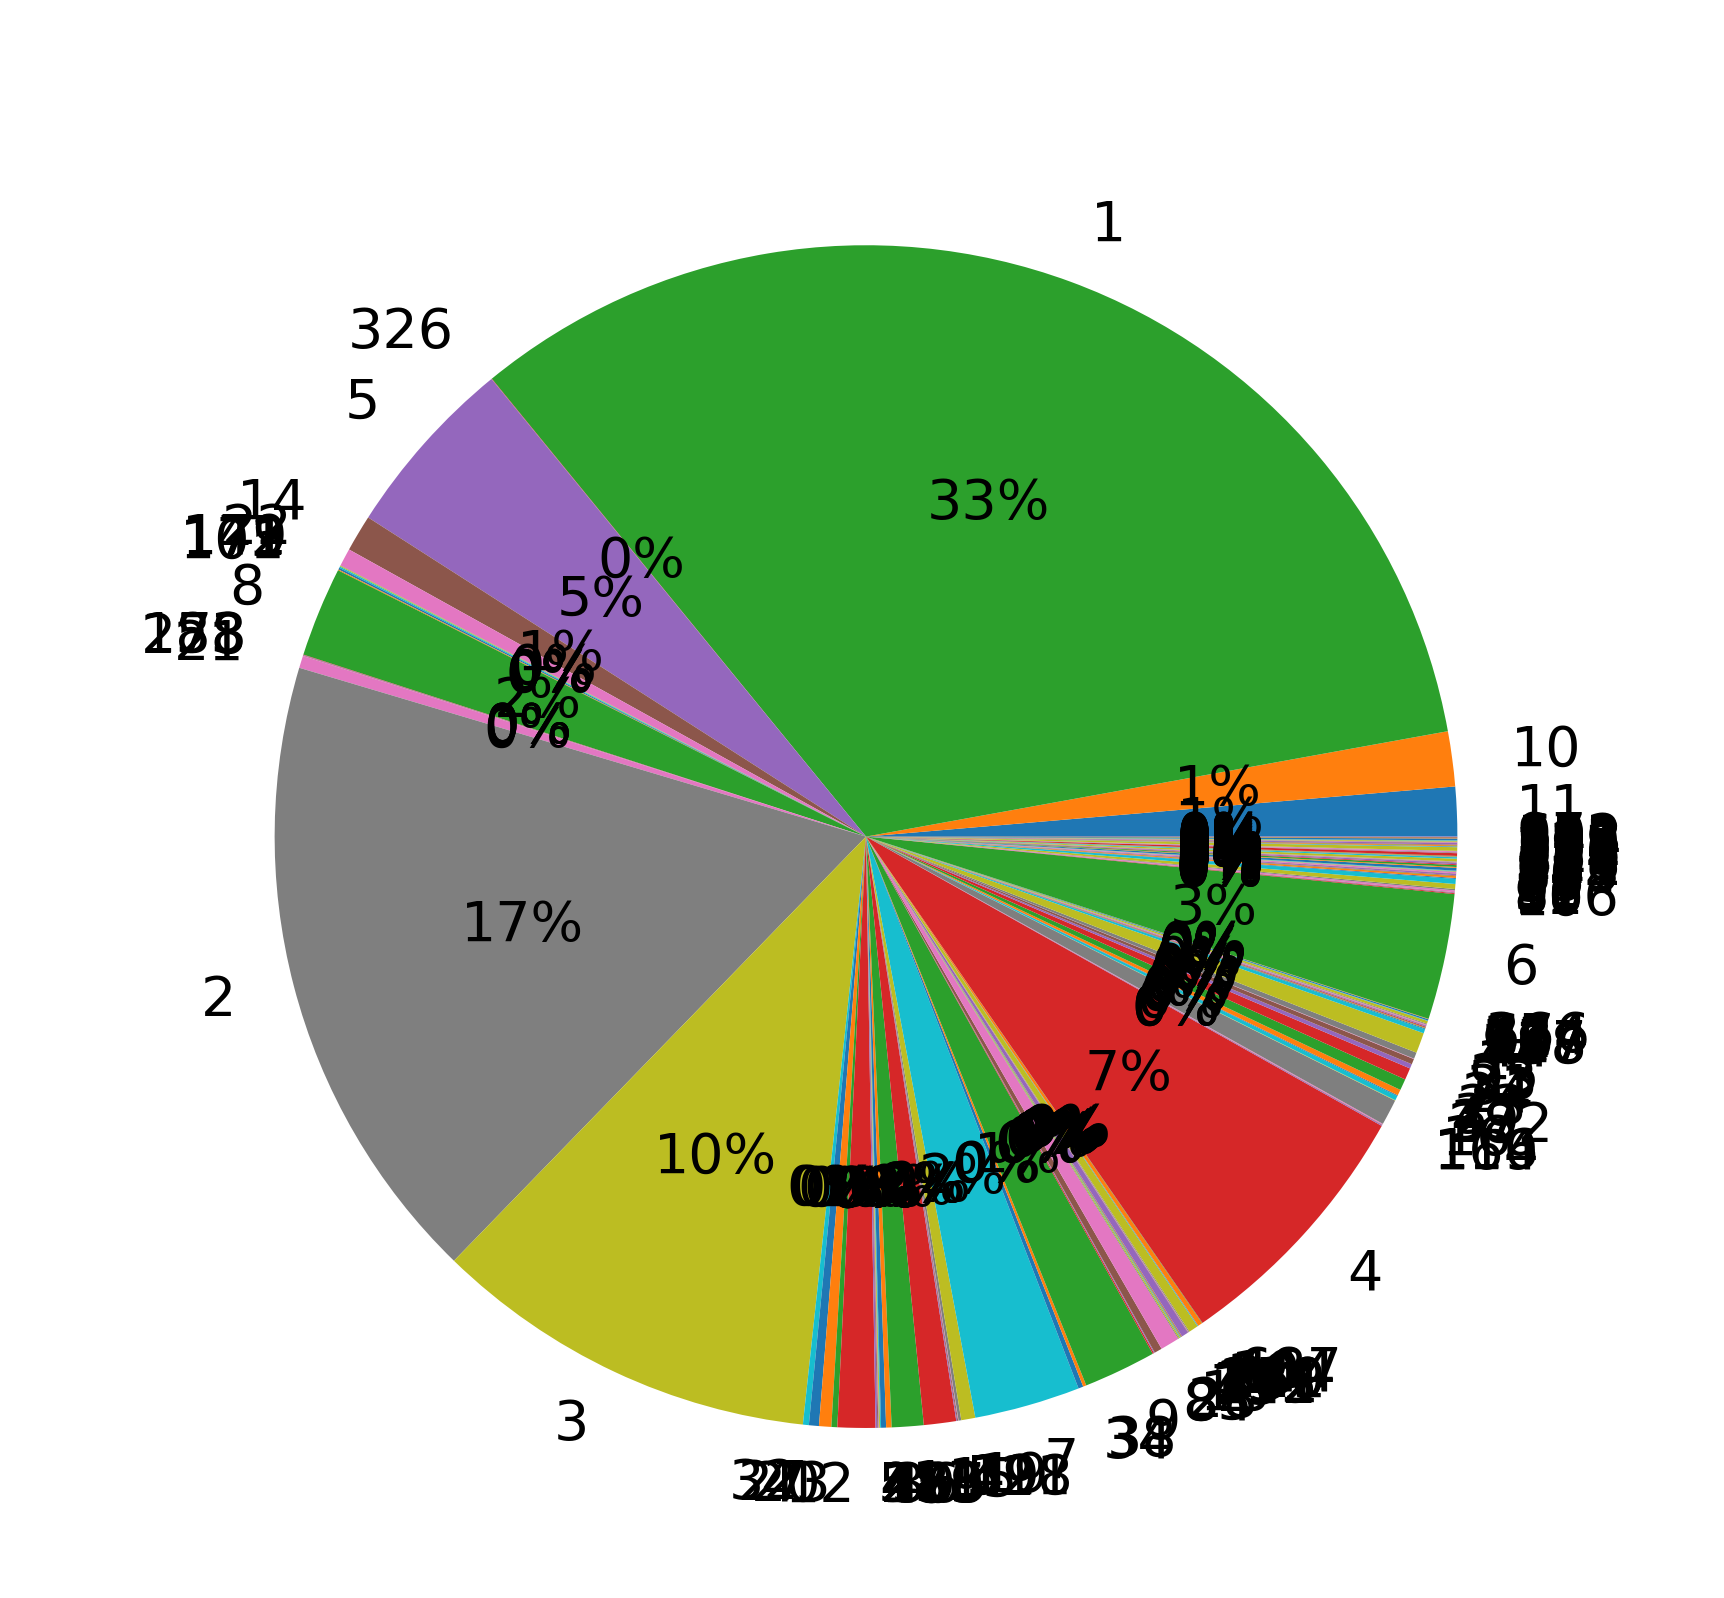
\includegraphics[width=2.3in]{../test_visualization_item}
        \caption{test\_item}
      \end{minipage}
    }
    \end{figure}
  \end{frame}
  \begin{frame}{User-Count Chart}
    \begin{figure}
    \centering
    \subfigure{
      \begin{minipage}{0.45\linewidth}
        \centering
        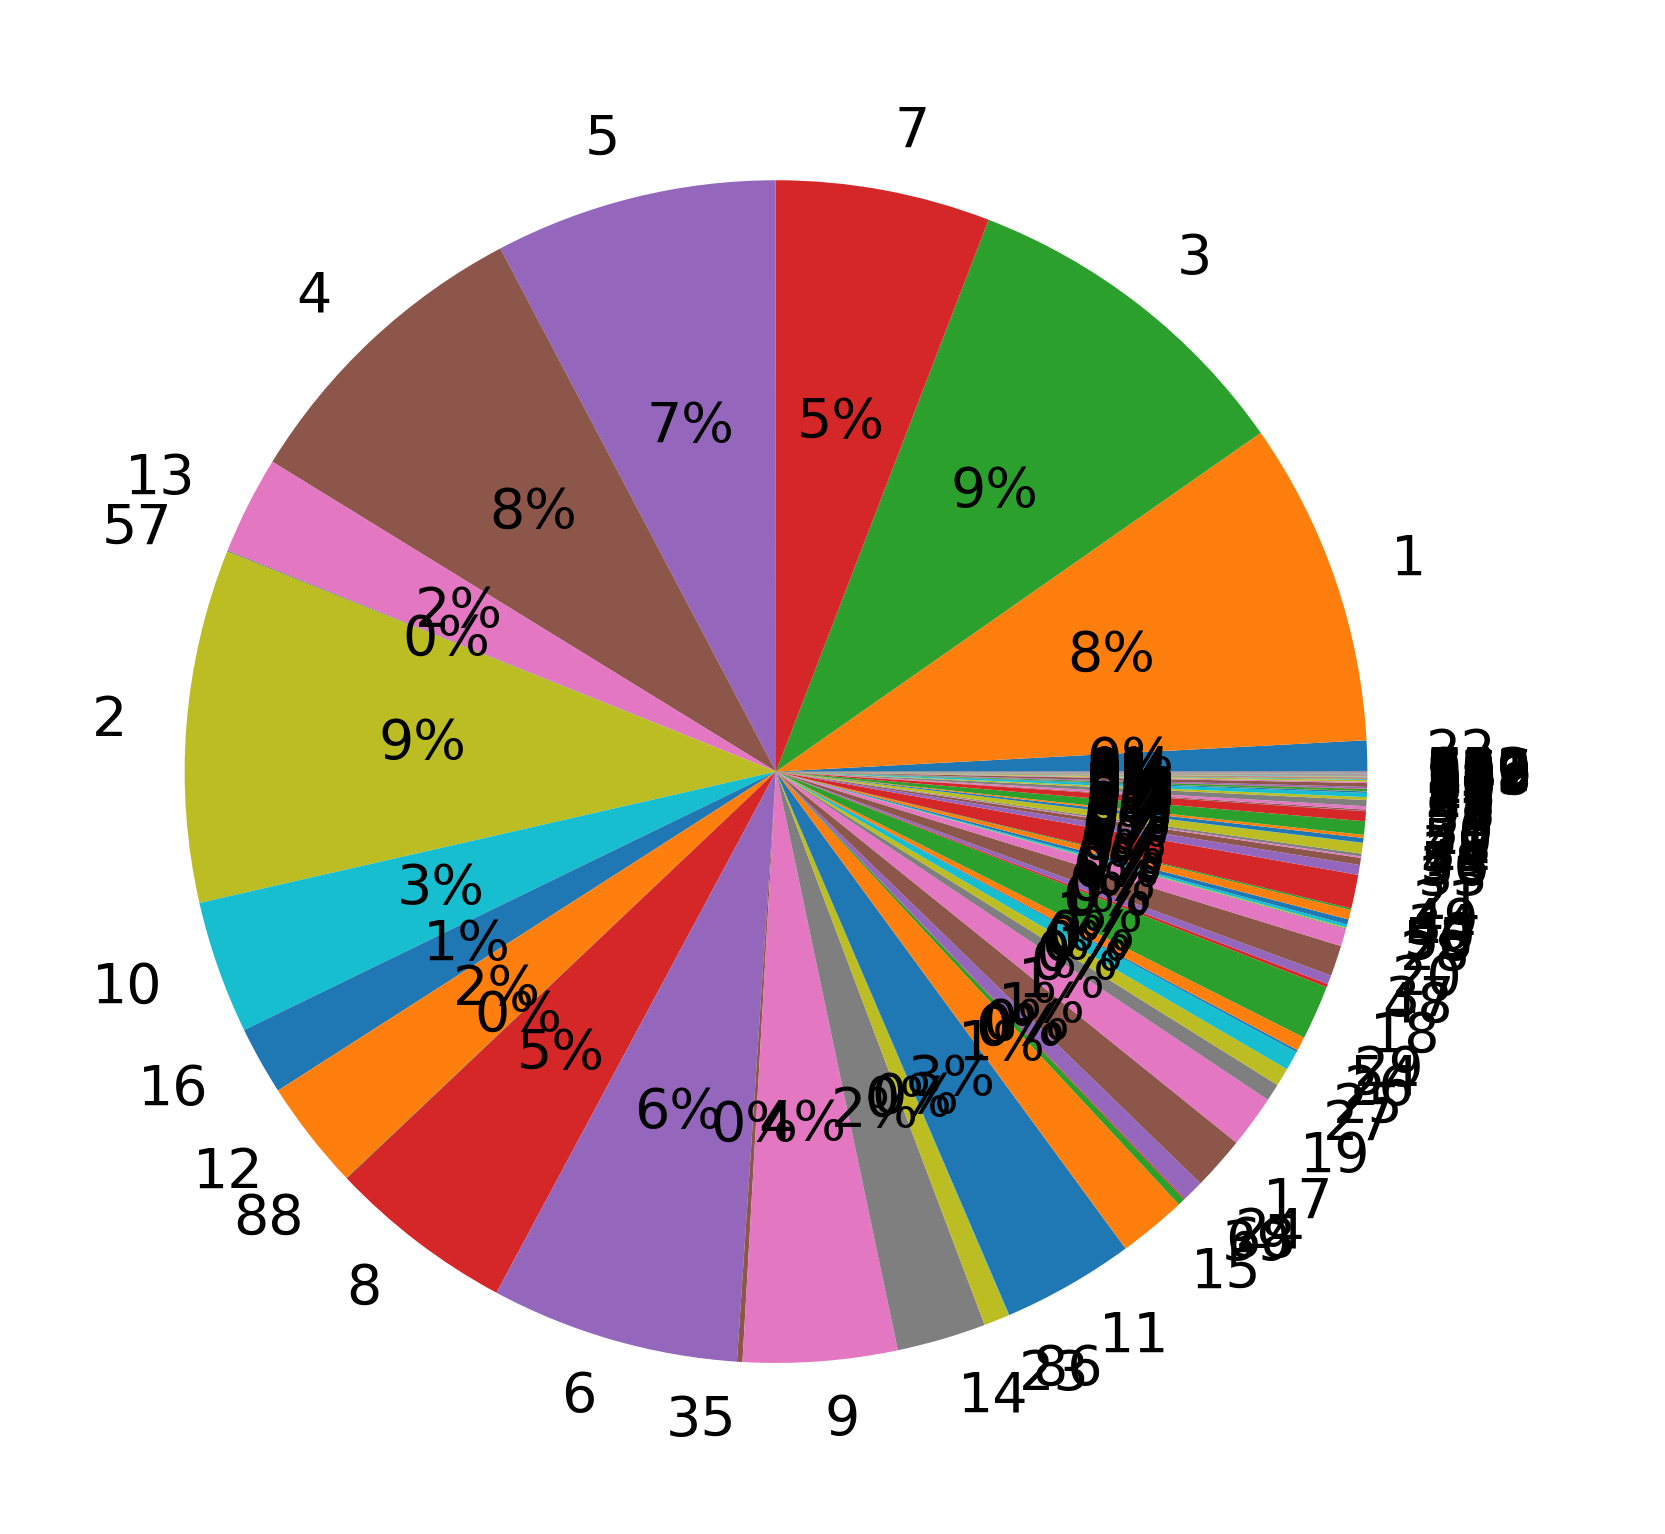
\includegraphics[width=2.3in]{../train_visualization_user}
        \caption{train\_user}
      \end{minipage}
    }
    \subfigure{
      \begin{minipage}{0.45\linewidth}
        \centering
        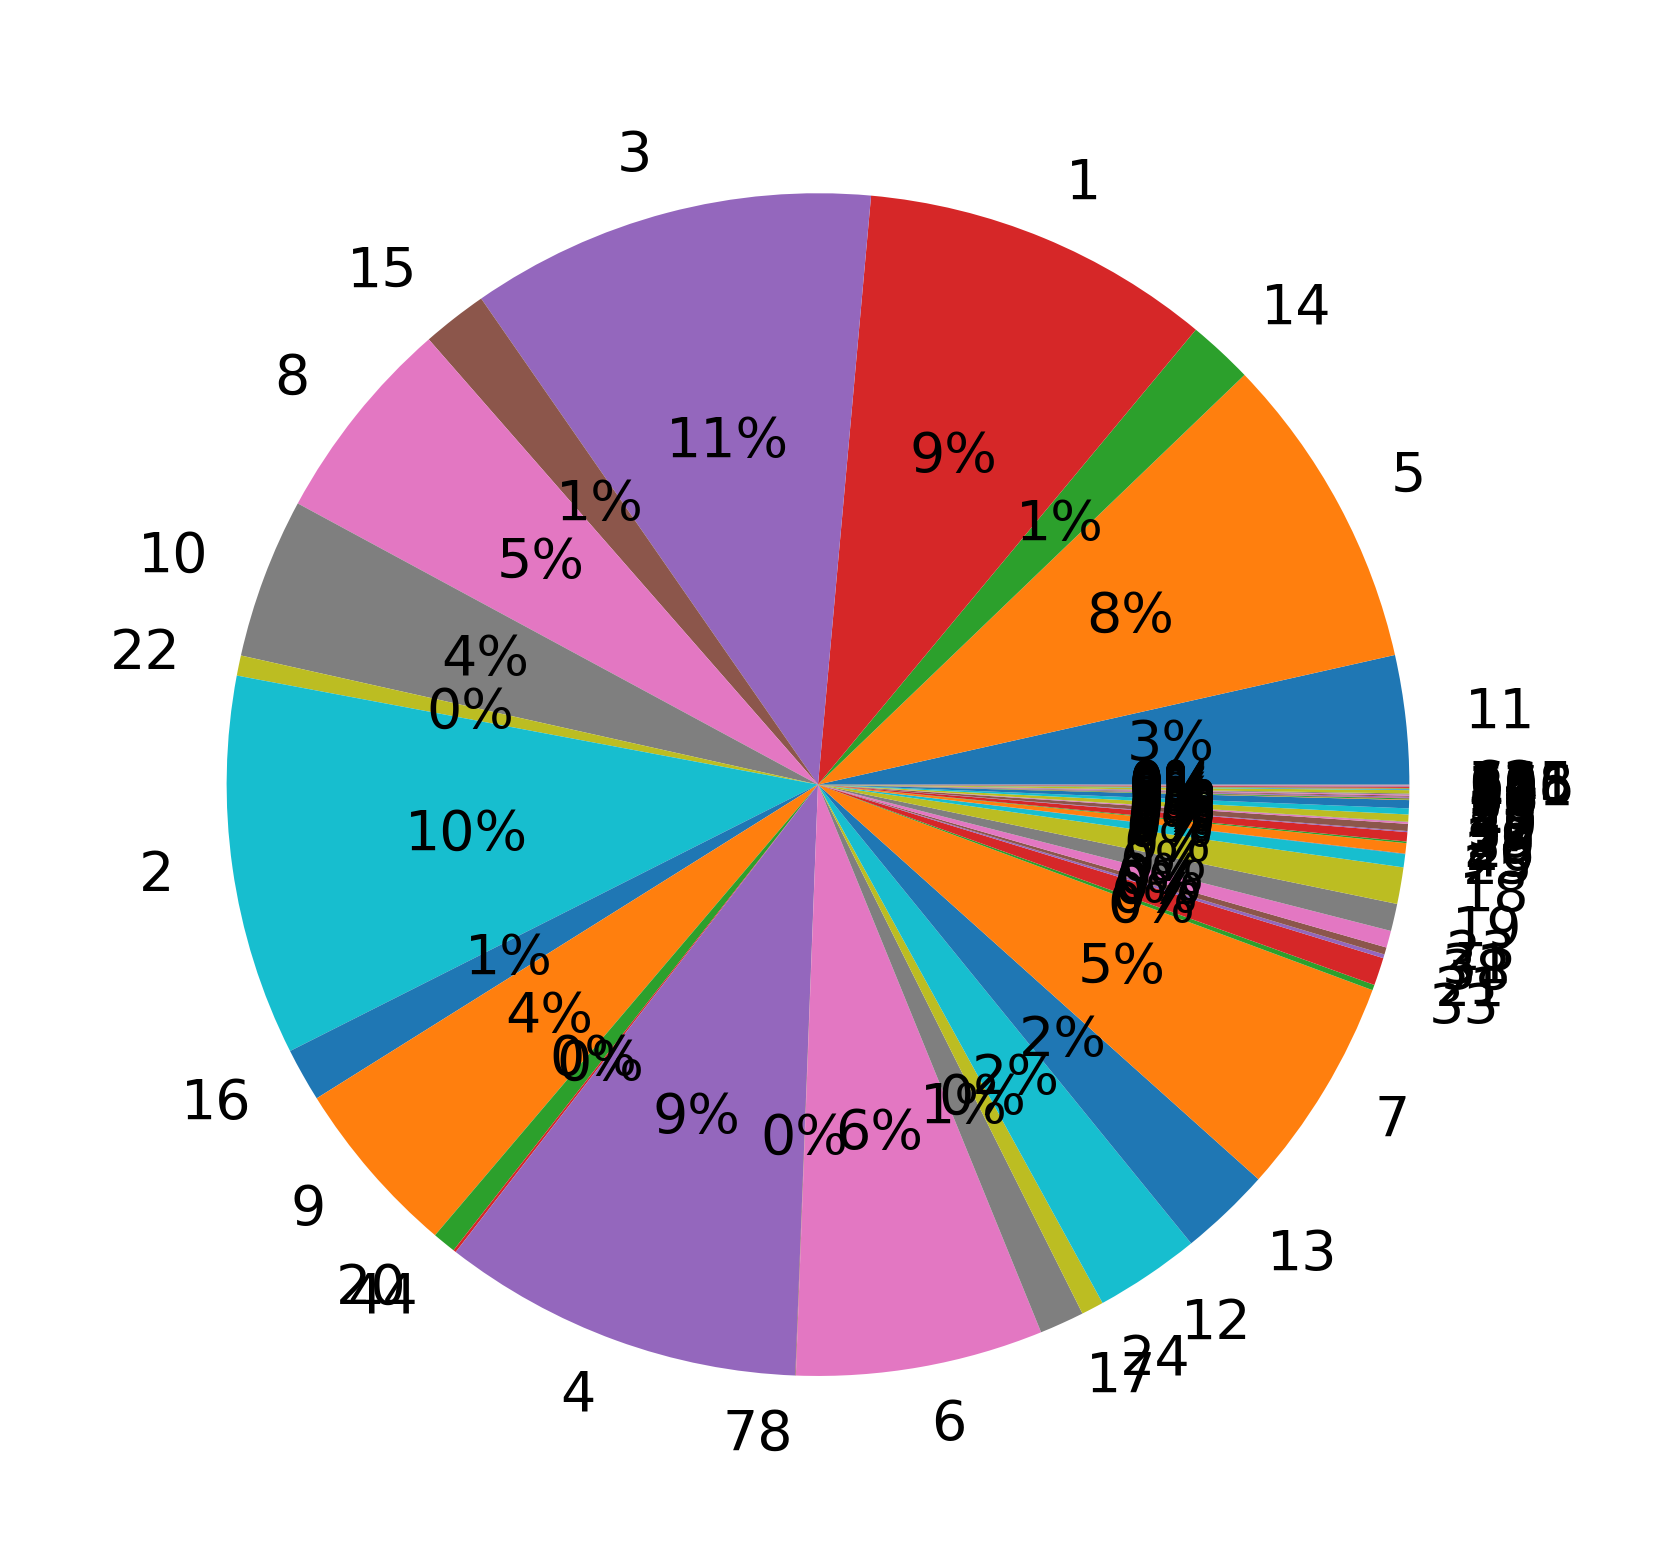
\includegraphics[width=2.3in]{../test_visualization_user}
        \caption{test\_user}
      \end{minipage}
    }
    \end{figure}
  \end{frame}
  
  
  \section{Improvement}
  \begin{frame}{Achievement}
    \begin{itemize}
      \item 更新了数据集, 使用了三个月的训练数据
      \begin{itemize}
        \item 相较于上次实验结果, 本次测试结果出现下降
      \end{itemize}
      \item 变化了测试时用户购买商品的种数的阈值
      \item 对于训练集未出现的商品, 在测试集中予以删除
      \begin{itemize}
        \item 可预料地, 提高了recall, 而precision不变
      \end{itemize}
      \item 根据用户测试集中购买的商品种数, 进行推荐(上限为$20$)
      \begin{itemize}
        \item 可预料地, 提高了precision, 而recall不变
      \end{itemize}
    \end{itemize}
  \end{frame}
  
  \begin{frame}{Result}
    \begin{figure}
      \centering
      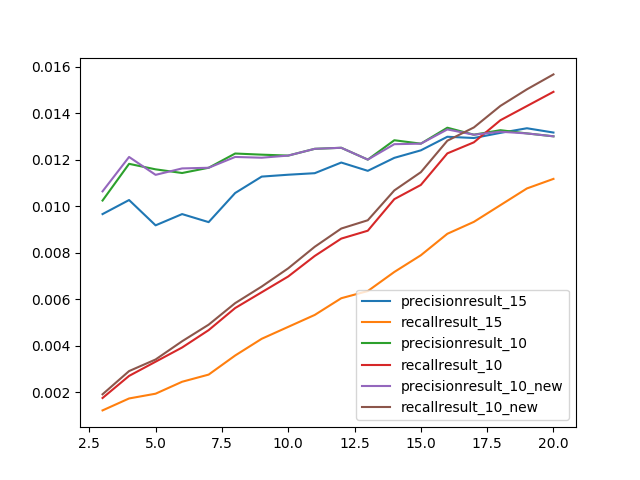
\includegraphics[width=\linewidth]{../result.png}
      \caption{precision\&recall}
    \end{figure}
  \end{frame}
  
  \begin{frame}{Dive into individual}
    Take User $13021568889$ for example
    \begin{itemize}
      \item In the Training
    \end{itemize}
    \centering\begin{tabular}{c | c | c | c | c}
      item & item\_id & count & amt & price\\
      \hline
      伊利lifeup红枣风味酸奶260g & 15114035 & 2 & 2.0 & 13.8\\
      花色小面包 & 23110004 & 2 & 7.98 & 7.98\\
      鲜到家黑椒牛排 & 24401037 & 1 & 0.196 & 23.48\\
    \end{tabular}
    \begin{itemize}
      \item In the Recommendation
    \end{itemize}
    \centering\begin{tabular}{c | c }
    item & item\_id\\
    \hline
    片仔癀牙火清牙膏(甄选留兰香)145g & 11301138\\
    益达纤柔焕彩牙刷(情侣装) & 11303197\\
    海太菠萝果粒果汁饮料238ml & 10119128\\
    \end{tabular}
  \end{frame}
  
  \begin{frame}  
    \begin{itemize}
      \item In the Test
    \end{itemize}
    \centering\begin{tabular}{c | c | c | c | c}
      item & item\_id & count & amt & price\\
      \hline
      七度空间公主系列卫生巾5片 & 11501062 & 1 & 1.0 & 9.9\\
      苏菲裸感S夜用29cm12片 & 11501116 & 1 & 1.0 & 15.8\\
      格力高百利滋蓝莓芝士45g & 14050013 & 1 & 1.0 & 3.9\\
      达利园瑞士卷巧克力味22g*10 & 14070003 & 1 & 1.0 & 6.9\\
      盼盼小面包奶香味440g & 14072017 & 1 & 1.0 & 10.9\\
      甘汁园阿胶红糖350g & 14863006 & 2 & 2.0 & 19.6\\
      蒙牛冠益乳原味/草莓果粒450g & 15115013 & 1 & 2.0 & 27.8\\
      蓝莓(大果/甜) & 22007031 & 1 & 0.64 & 12.8\\
      鱿鱼串 & 24220050 & 1 & 0.264 & 10.51\\
      儿童牛排 & 24401031 & 1 & 0.108 & 12.92\\
      鲜到家黑椒牛排 & 24401037 & 1 & 0.108 & 12.94\\
      包菜肉包 & 25111045 & 1 & 4.0 & 4.0\\
      酱菜系列 & 27100542 & 2 & 0.498 & 8.48\\
      山楂糕 & 27410044 & 1 & 0.244 & 4.83\\
    \end{tabular}
  \end{frame}

\end{document}
